\section{Quarterly vintage forecasts}
The 2020 edition supplies 1,615,443 approved \sba{} records and 187,255 approved 504 records. The dated-entry rule retains 1,352,814 and 108,606, respectively, across the full archive. The \sba{} file has 208,215 records missing an entry or approval date and 54,414 outside the entry window. The corresponding 504 counts are 33,114 and 45,535. The main scored vintages run from 1999Q1 through 2015Q4. They contain 883,104 \sba{} and 74,302 504 records across 68 quarters per program. Earlier records train the initial forecasts. The five-year incidence ranges from 2.93\% to 30.23\% in \sba{} and from 0.34\% to 14.94\% in 504. Adding every undated flagged charge-off to the horizon would increase a scored portfolio's incidence by at most 0.011 pp in \sba{} and zero in 504.
\begin{table}[htbp]
\centering\small
\caption{Error at the eight-quarter landmark, percentage points. The overlap column reports mean absolute error (MAE) for portfolios whose remaining observation window intersects 2007Q4--2009Q2. Maximum shortfall is the largest realized incidence minus forecast over all scored vintages.}
\label{tab:accuracy}
\begin{tabular}{lrrrrrr}
\toprule
 & \multicolumn{3}{c}{7(a)} & \multicolumn{3}{c}{504} \\
\cmidrule(lr){2-4}\cmidrule(lr){5-7}
Method & MAE & Overlap & Max. shortfall & MAE & Overlap & Max. shortfall \\
\midrule
\tableinput accuracy.tex
\bottomrule
\end{tabular}
\end{table}
Using the latest available age-specific increments reduces mean absolute error by 1.28 pp in \sba{} and 0.75 pp in 504 (Table~\ref{tab:accuracy}). The period window beats the mature window in 40 and 44 of 68 quarterly comparisons, respectively. The eight-quarter block resampling ranges for period minus mature MAE are $[-3.99,1.09]$ and $[-1.81,0.08]$ pp. In \sba{} the range spans zero for all three block lengths. In 504 its upper endpoint is close to zero for blocks of four and twelve. These ranges summarize sensitivity to which contiguous portfolios are resampled. The blocks span at most twelve quarters and successive forecasts share donors and targets for longer. The ranges cannot quantify uncertainty across independent economic cycles.

The freshness comparison goes the other way for multiplicative development. Allowing new vintages into the successive development factors raises average error by 0.28 pp in \sba{} and 2.24 pp in 504. One 504 chain forecast reaches the 100\% cap. For the 2007Q4 vintage it scales an early incidence of 2.05\% to the cap against a realized 13.00\%. Across leave-one-quarter-out summaries the 504 chain still increases MAE by 1.10 to 2.52 pp relative to the mature factor. Sparse early events can make the product unstable. In \sba{} the mature factor gives the lowest overall MAE, while the single-vintage additive forecast has the lowest MAE in 504. The latter benefits from newer data but also carries greater quarter-specific variation.

The length of the information window matters independently of vintage eligibility. At four and twelve quarters, respectively, period MAE is 4.80 and 5.53 pp for \sba{} and 2.88 and 3.47 pp for 504. Mature increments are less accurate at both widths in both programs. Within short and long term groups, the eight-quarter period window also has lower MAE than mature increments. The reductions are 1.38 and 0.18 pp in \sba{}, and 0.11 and 0.77 pp in 504. Some short-term 504 portfolios lack a nonzero denominator for fitting multiplicative development. All additive forecasts are defined.
\begin{figure}[htbp]
\centering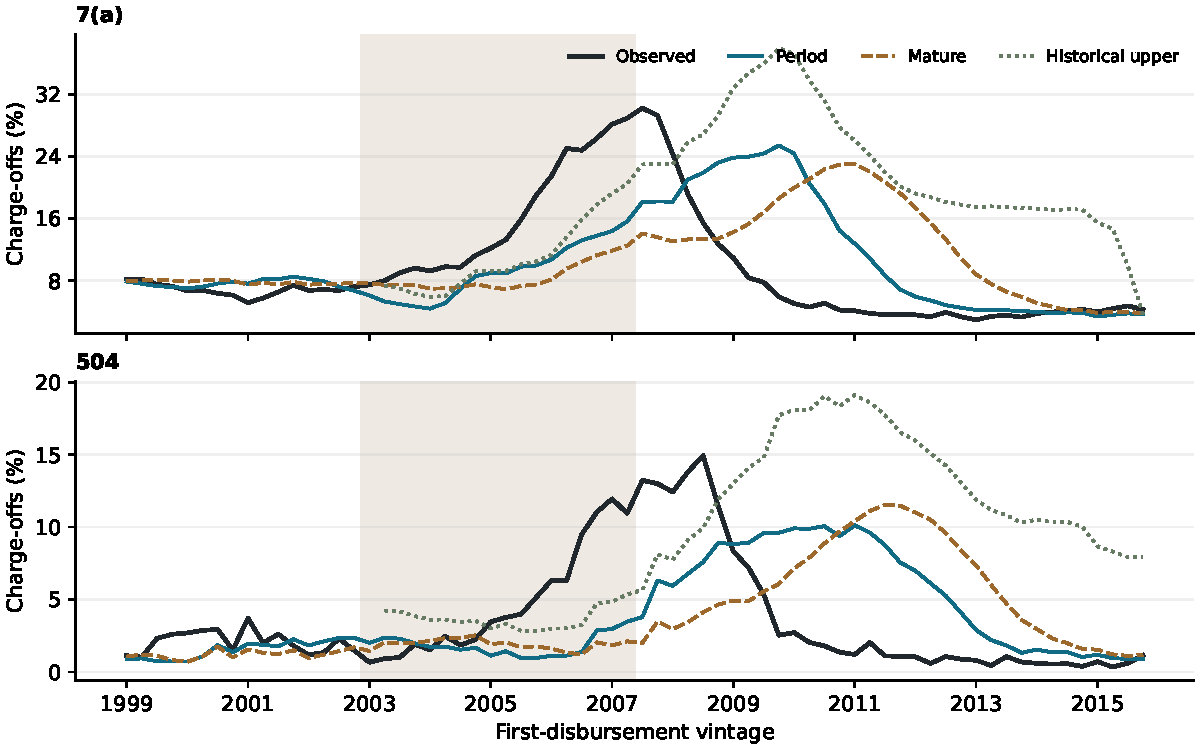
\includegraphics[width=.96\linewidth]{vintages.pdf}
\caption{Dated charge-offs over the first twenty quarters, ordered by disbursement vintage. The shaded vintages have a post-landmark window that overlaps the financial crisis. Each line at a given vintage forecasts the same endpoint from an eight-quarter prefix, except the observed series which uses the mature outcome.}
\label{fig:vintage}
\end{figure}

\subsection{How often did the upper forecasts hold?}
\begin{table}[htbp]
\centering\small
\caption{Historical margins and multiplicative stress scenarios. Covered gives the count below or at the historical upper forecast. Margin and breach are the mean addition above the point forecast and the largest amount above the historical upper forecast, respectively, in pp. Double counts outcomes at or below a doubled tail. Inside counts those between a halved and a doubled tail.}
\label{tab:upper}
\begin{tabular}{llrrrrrr}
\toprule
Program & Window & $n$ & Covered & Margin & Breach & Double & Inside \\
\midrule\tableinput upper.tex
\bottomrule
\end{tabular}
\end{table}
Eighteen vintages per program have a tail that overlaps the financial crisis. Seventeen have the twenty mature forecast errors required to issue the historical upper forecast. In \sba{}, none of these seventeen outcomes falls below or at the upper forecast. The mean addition to the point estimate is only 1.71 pp in that subset, compared with 10.85 pp outside it. Even a doubled forecast tail covers only six of the seventeen outcomes. The 504 upper forecast covers seven of seventeen. These are adjacent vintages exposed to one crisis, so the seventeen misses in \sba{} describe a sustained failure in time.

The error changes direction as older stressed vintages enter the reference set (Figure~\ref{fig:vintage}). For \sba{} disbursements in 2009Q4, the period forecast is 25.42\% against an outcome of 5.90\%. This overprediction and the earlier underpredictions have different implications for a lender estimating future charge-off counts. A mean signed error near zero can coexist with large shortfalls on one side of the cycle. Table~\ref{tab:upper} reports both nonexceedance and the cost of carrying the margin.

\section{Matched weights and a later disbursement panel}

The primary comparison gives equal weight to donor vintages for increments and pools loan counts for the development factors. We repeat both rules with a common weighting convention throughout. For donor cohort $u$ let $w_u$ sum to one within each age-specific pool, using equal weights or weights proportional to the number of funded loans. Write $d_j=\sum_u w_u x_{uj}$ and $b_j=\sum_u w_u F_u(j-1)$. An additive forecast transfers $d_j$ at each remaining age. A multiplicative forecast uses $1+d_j/b_j$. We hold the weighting convention fixed when moving both quantities to recent donors. Every reported comparison uses the same target quarters for the two windows and the two families.

\begin{table}[htbp]
\centering\small
\caption{Recent minus mature MAE (pp) with matched donor weights at age eight. Positive values favor mature donors. The exclusion row retains quarters for which the full donor and target span avoids the financial crisis. Later quarters are disjoint from the original disbursement panel.}
\label{tab:transfer}
\begin{tabular}{llr rrrr}
\toprule
 & & & \multicolumn{2}{c}{Equal vintage weights} & \multicolumn{2}{c}{Loan weights} \\
\cmidrule(lr){4-5}\cmidrule(lr){6-7}
Program & Panel & $n$ & Add & Multiply & Add & Multiply \\
\midrule\tableinput matched.tex
\bottomrule
\end{tabular}
\end{table}

In the full original panel the sign difference across forecast families survives both weighting conventions (Table~\ref{tab:transfer}). Its economic magnitude is sensitive to the years included. At the fixed landmark the earliest donor event that can enter a development factor is in quarter $v-19$ and the last scored event is in $v+19$. Excluding portfolios for which any quarter of that span intersects 2007Q4--2009Q2 leaves 23 quarters in each program. The 7(a) additive advantage of 1.28 pp becomes a disadvantage of 0.04 pp. In 504, the additive advantage shrinks from 0.75 to 0.14 pp. This exclusion also removes the surrounding years and cannot identify a causal recession effect.

Using the September 2025 edition, we score all fifteen subsequent quarterly vintages with complete common coverage (2016Q1--2019Q3), comprising 195,691 \sba{} and 12,477 504 records. We apply the same date mask and age-eight landmark, without tuning a window on these portfolios. With equal donor weights, recent increments improve MAE by 0.15 pp for \sba{} and give up 0.01 pp in 504. Recent development factors increase error in both programs. The 504 file alone supports five further vintages, 2019Q4--2020Q4. There the recent additive window gains 0.26 pp while the two multiplicative forecasts tie on average. We keep these five outside the common comparison.

\paragraph{What changes in a development factor?}
Let $L_{ij}$ denote MAE after choosing the source of increments $i$ and of the cumulative base $j$ separately, each mature ($M$) or recent ($R$). The forecasts retain the original prefix and cap. Following the order-averaged decomposition in Shorrocks \cite{shorrocks}, the increment contribution is $[(L_{RM}-L_{MM})+(L_{RR}-L_{MR})]/2$. Subtracting this from $L_{RR}-L_{MM}$ gives the base contribution. In the original \sba{} panel, with loan weights, the net 0.28 pp increase comprises $+3.22$ pp from updating increments and $-2.94$ pp from updating the cumulative base. In 504 the corresponding terms are $+3.69$ and $-1.46$ pp. The latter portfolio's subsequent common panel gives $-0.02$ and $+0.37$ pp. The hybrid substitutions describe the mechanics of the recorded loss difference. The offset in the historical aggregates does not fix its sign or size elsewhere.

\paragraph{Other US recession windows.}
We use the calendar quarters containing the NBER monthly peak and trough. As before, a target qualifies if any of its twelve remaining quarters overlaps the episode. To preserve the original error history, calibration uses mature errors from the original replay through the 2015Q4 disbursement vintage, then from the later replay. These are retrospective, date-masked errors. Four scored portfolios per program overlap the 2001 downturn but none has twenty mature historical errors, so upper-forecast coverage is unobservable there. For the 2020 downturn (2020Q1--Q2), the historical period upper forecast covers seven of thirteen eligible \sba{} outcomes and ten of thirteen 504 outcomes. In 2007--09 it covered zero and seven of seventeen, respectively. SBA payment relief for eligible outstanding loans during the pandemic changed the setting \cite{relief}. Each count describes one sequence of overlapping portfolios within one macroeconomic episode.

\section{Does reconstructing the archive change the ranking?}
For an early edition $e$ and the 2025 edition $f$, write $\widehat R^{e}$ for the projected additional incidence. The reporting contribution and tail error can be measured separately:
\[
F_v^f(H)-\widehat F_v^e(H)
 = \big[F_v^f(a)-F_v^e(a)\big] +
   \big[F_v^f(H)-F_v^f(a)-\widehat R^e\big].
\]
Rates use the denominator in their respective editions. The first term captures net changes to eligible records and to dates that fall before the cutoff. Opposing revisions can cancel at the portfolio level. In a further check we rebuild the period forecast from the 2025 file, masking all events after the earlier origin. The difference from the archived forecast also captures revisions to the donor histories. Entry support is checked separately for each source and scoring file. The 7(a) final slice ends with FY2019 approvals. We stop at 2019Q3 disbursements to avoid partially observed portfolios. Both September 2022 and September 2025 have continuing 504 files, which also support the later 504 vintages. Donor coverage is complete for all retained targets under the 365-day entry rule.

Define $D_e$ as MAE with the recent window minus MAE with the mature window, calculated using archived inputs and the 2025 outcomes. Define $D_f$ identically after reconstructing both forecasts from the 2025 file with the historical event-date mask. Lower error for recent vintages gives a negative difference. Scoring the identical outcomes at identical ages makes $D_f-D_e$ an input-edition effect on the comparison. For reference, the triangle inequality bounds its magnitude by the mean sum of the absolute revisions in the two forecasts. A gap larger in magnitude than that bound must retain its sign. Individual revisions and bounds are included in the supplement.

\begin{table}[htbp]
\centering\small
\caption{Does the recent window have lower MAE? Differences are recent minus mature MAE in pp, across all supported portfolio ages at each origin. Archived columns use the actual earlier file. Replay columns use date-masked September 2025 inputs. A change in sign reverses the ranking.}
\label{tab:external}
\begin{tabular}{llrr rrrr}
\toprule
 & & & & \multicolumn{2}{c}{Additive} & \multicolumn{2}{c}{Multiplicative} \\
\cmidrule(lr){5-6}\cmidrule(lr){7-8}
As of & Program & Ages & $n$ & Archived & Replay & Archived & Replay \\
\midrule\tableinput external.tex
\bottomrule
\end{tabular}
\end{table}

In the September 2020 \sba{} file, using recent development factors improves MAE by 0.185 pp. Reconstructing the same forecasts from the 2025 file gives the mature factors a 0.215 pp advantage (Table~\ref{tab:external}). The gap moves by 0.400 pp with the scoring outcomes fixed. Two other multiplicative comparisons also change sign, including a 504 gap below 0.01 pp in either direction. The September 2022 504 forecasts give identical archived and reconstructed gaps. These five program--origin pairs share programs, economic conditions and final outcomes. Three reversals are descriptive cases.

\paragraph{Comparison at the primary landmark.}
Only three program--origin pairs support an eight-quarter forecast scored at twenty quarters. In September 2020, the archived additive gap is $-0.010$ pp for \sba{} and $+0.036$ pp for 504. In September 2022 it is $-0.282$ pp for 504. The September 2020 \sba{} gap becomes $+0.066$ pp in the masked replay. Each figure concerns one portfolio. The 2022 \sba{} files cannot supply the later fully represented disbursement quarters required at age eight. Consequently the pooled-age rows in Table~\ref{tab:external} evaluate a mix of remaining horizons and cannot serve as replications of the two-year-landmark result. The two 2022 origins are one quarter apart. Archive as-of dates establish what the files contained. Contemporaneous public access on those exact dates is unverified, which matters especially at a one-quarter remaining horizon.

In the twelve September 2020 \sba{} portfolios, the mean prefix subsequently falls by 0.222 pp while the realized post-landmark increment exceeds its period forecast by 0.116 pp. These components partly offset. The denominator also moves from 161,863 to 162,046 records. In the six December 2022 \sba{} portfolios the mean prefix revision is $-0.112$ pp and mean tail error is $-0.256$ pp. Reconstructing that period forecast from the 2025 edition would report MAE of 0.210 pp in place of 0.368 pp. The aggregate comparison cannot assign the revisions to individual loans.
